\begin{frame}
    \frametitle{Network Architecture}
    
    \begin{columns}[T]
        \begin{column}{0.4\textwidth}
            \begin{alertblock}{Model}
                \begin{itemize}
                    \item $\num{4}$ Dense Layers with Dropout
                    \item Loss function: categorical crossentropy
                    \item Optimizer: adam
                \end{itemize}    
            \end{alertblock}
        \end{column}
        \begin{column}{0.6\textwidth}
            \begin{figure}
                \hspace*{-1.7cm}
                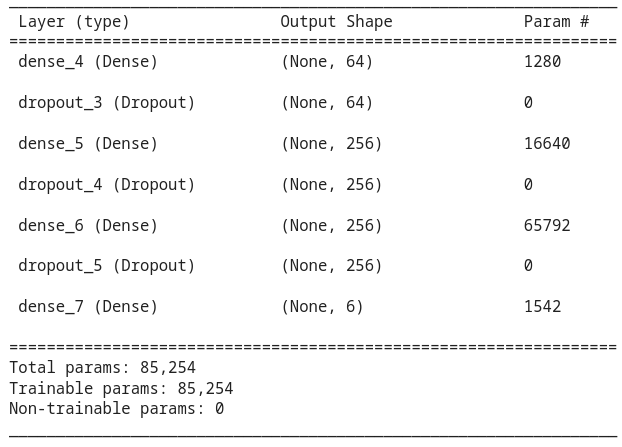
\includegraphics[width=1\textwidth]{../figures/model_summary.png}
            \end{figure}
        \end{column}
    \end{columns}

    \begin{alertblock}{Training}
        \begin{itemize}
            \item Early stopping: Stops training when the validation loss function no longer improves
            \item Reduce learning rate: Decreases learning rate if validation loss function stagnates \\
            \to better convergence
            \item Train the model using the training data with the defined set of hyperparameters.
        \end{itemize}  
    \end{alertblock}
    
\end{frame}
    